\documentclass[oneside]{book}

\usepackage[
  top=1.25in,
  bottom=1.25in,
  left=1.25in,
  right=1.25in,
  bindingoffset=0.25in,
  heightrounded,
]{geometry}

\usepackage{tabularx}
\usepackage{listings}
\usepackage{float}
\usepackage{graphicx}

\graphicspath{ {images/} }

%\title{Library Box}
%\date{2020-12-10}
%\author{Andrea Calici (10490117)}

\begin{document}

\begin{titlepage}
\centering
\vspace*{\stretch{1}}

\includegraphics[scale = 0.3]{logo.png}

{\LARGE A.Y. 2020/2021\par}

%\vspace*{\stretch{1}}
{\LARGE Design and Implementation of Mobile Applications\par}
%\vspace{2cm}
{\LARGE Library Box\par}
{\LARGE Design Document\par}
%\vspace{1cm}
{\large Andrea Calici (10490117))\par}
\vspace*{\stretch{2}}
\end{titlepage}

%\maketitle
\pagenumbering{gobble}

\tableofcontents
\newpage

\pagenumbering{arabic}

\chapter{Introduction}
\section{Purpose}
The aim of this document is to describe the design and the implementation of a mobile and web application developed for Android and the most common web browsers through the functional description of the system, a detailed analysis of its architecture, its components and the way they interact.\newline
Starting from the work developed by Medici Volontari Italiani with the Carta d'Identità Salvavita and the Busta Rossa project of Comune di Milano, I and Davide Laffi developed a system that is able to:

\section{State of the Art}
At the moment the are a lot of different systems that are used to fulfill the same goal: the safeguard for the health of the citizens. In fact a single patient:
\begin{itemize}
\item has his Personal Health Record that is available in the site of the region of residence;
\item has his Individual Medical Record written by his doctor;
\item can use the ICE application in order to contact the health autorities;
\item can request the Carta d'Identità Salvavita by Medici Volontari Italiani.
\end{itemize}
Obviously the are many duplicate information, proprietary systems, data that are manually inserted, updated and lost.

\subsection{Carta d'Identità Salvavita}
Medici Volontari Italiani developed, with the help of Fondazione IBM, Società Gisette and Comune di Milano, a system that allows to digitalize life-saving health data through the digital version of the Carta d'Identità Salvavita (C.I.S.).\newline
The C.I.S. is a document that displays:
\begin{itemize}
\item personal details;
\item phone numbers that can be called in case of emergency (I.C.E. numbers);
\item life-saving data.
\end{itemize}
All this data can be 

\section{Scope}
The main goal of this thesis is to develop a system that can unify all the characteristics defined above in order to create a single flow that starts from the data entry realized by the doctor and the volunteer and ends in a mobile application where the end-user (the citizen) is able to check is data.

\subsection{Goals}
The main goals of the application are the followings:

\subsubsection{Citizen}
\paragraph{[G1]} Allow a citizen to become user of the application following the entering of his data by the doctor or the volunteer;
\paragraph{[G2]} Allow an user to login to the system after providing valid credentials (email and password);
\paragraph{[G3]} Display to the user the QR code that summarizes his life-saving information and allow him to open, save and print it;
\paragraph{[G4]} Display to the user his Patient Summary, his Carta d'Identità Salvavita, his badge and his bracelet and allow him to open, save and print them;
\paragraph{[G5]} Display to the user his Covid history through a QR code and a list of entry (swabs and vaccination) that describe his situation and allow him to open, save and print them;
\paragraph{[G6]} Allow an user to contact his doctor and the volunteer that filled out his data through email or phone number;

\subsubsection{Volunteer}
\paragraph{[G7]} Allow a volunteer to login to the system after providing valid credentials (email and password);
\paragraph{[G8]} Allow a volunteer to search through the citizens of his jurisdiction;
\paragraph{[G9]} Allow a volunteer to print the Carta d'Indentità Salvavita, the badge or the bracelet of a particular citizen;
\paragraph{[G10]} Allow a volunteer to print multiple Carte d'Identità Salvavita, badges or bracelets.

\subsubsection{Generic}
\paragraph{[G11]} Allow an user to reset his passwords;
\paragraph{[G12]} Display a list of emergency numbers that can be called in case of necessity;
\paragraph{[G13]} Allow an user to scan a QR code to show the data of a particular citizen.

\section{Definitions and Acronyms}
\subsection{Definitions}

\subsection{Acronyms}


\chapter{Project Overview}
\section{Introduction}
The whole project is composed of three main parts that will be described in details in the next sections:
\begin{itemize}
\item web application;
\item database;
\item mobile application.
\end{itemize}

\subsection{Web Application}
The web application was developed by Davide Laffi and focuses on the data entry part for the entire system. There are two main actors involved in its use:
\begin{itemize}
\item the doctor that can compile the patient summary;
\item the volunteer allowed to insert personal data of the citizen.
\end{itemize}

\subsection{Database}

\subsection{Mobile Application}


\chapter{Implementation}
\section{Architecture}
The whole system can be divided in three main parts:
\begin{itemize}
\item the web application developed by Davide Laffi and intended to use by the doctor and the volunteer in order to fill out information of the citizens;
\item the database implemented using Google Firebase in order to store all the data of the citizens;
\item the mobile application developed by me using Flutter and intended to use by the citizens in order to access and use their data.
\end{itemize}

\section{Flutter}
\textbf{Flutter} is an open-source UI software development kit created by Google and released in 2017, used to develop cross-platform mobile applications. Flutter code is written in Dart, a client-optimized programming language for apps on multiple platforms also developed by Google and used to build not only mobile but also desktop, server, and web applications. Flutter has some very important characteristics that brought the decision of use this code language for the development of the application:
\begin{itemize}
\item \textbf{Cross-platform}: Flutter bases on Dart which is a unique language the allows to develop the same application for Android, iOS and the web;
\item \textbf{Firebase}: the integration between Flutter and Firebase is very simple and easy to implement. This is because Flutter is a Google coding language, while Firebase is a Google service. 
\item \textbf{Widgets}: user interface is made of composition of widgets which developers have to assembly and link together. Widget is a very powerful unit both on code and UI part.
\item \textbf{Plugins and Packages}: Flutter has a large community which supports it. This allows most expert users to release plugins which are external libraries which permit to implement and integrate lots of services.
\end{itemize}

\section{Web Application}
Breve riassunto sulla parte di Davide.

\section{Mobile Application}

\chapter{Functionalities}

\chapter{Discussions and Conclusion}
The system at the moment allows the doctor to enter his patients' information that can be accessed by the user of the application. The next step will be the integration of the system with other proprietary softwares, in particular:
\begin{itemize}
\item FSE;
\item app ICE.
\end{itemize}
\begin{figure}[H]
\centering
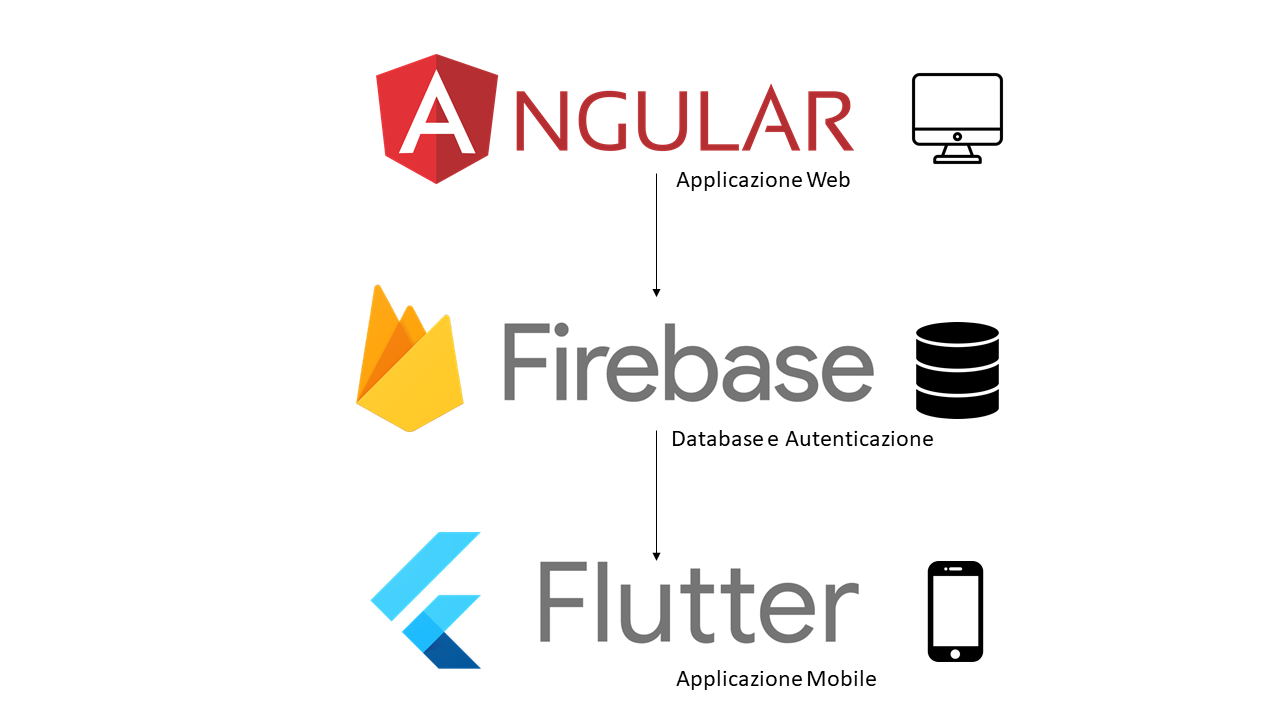
\includegraphics[scale = 0.3]{architecture}
\caption{The architecture of the application}
\end{figure}
\end{document}